\documentclass[a4paper]{article}
\usepackage[utf8]{inputenc}
\usepackage[spanish]{babel}
\usepackage{geometry}
\geometry{
	a4paper,
	total={170mm,257mm},
	margin=0pt
}
\usepackage{mathptmx}
\usepackage[hidelinks]{hyperref}
\usepackage[11pt]{extsizes}
\usepackage{graphicx}
\usepackage{caption}

\title{
	\fontfamily{phv}\selectfont
	\textbf{Diseño e implementación de un servicio de búsqueda multi-hilo}
}
\author{
	\fontfamily{phv}\selectfont
	Ángel Pérez Porras \\
	\fontfamily{phv}\selectfont
	E.S. de Informática, Universidad de Castilla-La Mancha \\ \\
	\fontfamily{phv}\selectfont
	\hyperref{mailto:angel.perez7@alu.uclm.es}{}{}{angel.perez7@alu.uclm.es}
}
\date{\fontfamily{phv}\selectfont Junio de 2021}

\makeatletter
\renewcommand\section{\@startsection {section}{1}{\z@}%
	{-3.5ex \@plus -1ex \@minus -.2ex}%
	{2.3ex \@plus.2ex}%
	{\normalfont\large\scshape}}
\makeatother
\captionsetup[figure]{labelfont={sc},labelsep=period}

\begin{document}
	\maketitle
	
	\begin{abstract}
		Para la tercera práctica de la asignatura de Sistemas Operativos II, se solicita el diseño e implementación de un programa en el lenguaje C++ siguiendo el paradigma productor-consumidor en el que se presta un servicio de búsqueda textual a clientes que lo solicitan de forma dinámica. En esta propuesta se implementan varios servicios que, mediante el paso de mensajes y utilizando características de concurrencia modernas de la librería estándar de C++, simulan peticiones de dichos servicios por parte de clientes que se crean continuamente. La solución se materializa en la producción de dos artefactos \textit{software}; a saber, un prototipo escrito en el lenguaje de programación Python (\texttt{protofind2.py}) y una implementación final del programa \texttt{mtfind2(1))} (haciendo alusión al producto de la práctica anterior).
	\end{abstract}

	\tableofcontents
	
	
	\section{Problema Planteado}
	El objetivo de la práctica es la implementación de un sistema complejo de búsqueda textual. En él, se involucran clientes y servicios mediante peticiones que utilizan unos recursos limitados (\textit{e.g.} de cómputo, de memoria...) y que deben ser gestionados de manera eficiente para evitar un eventual colapso de la plataforma en que se ejecuta, así como asegurar que se atiende a todos los clientes y no se produce inanición\footnote{El problema de la \textit{inanición} se da cuando, en un contexto de concurrencia, a un proceso se le deniega de manera continua el acceso a un recurso, de manera que no puede continuar su ejecución o no puede hacerlo de manera normal. Este problema indica un error en los algoritmos de planificación o un uso incorrecto de las facilidades de acceso concurrente (como semáforos o exclusión mutua).}.
	
	El sistema consiste en una simulación en la que muchos clientes, de manera concurrente, generan peticiones de búsqueda aleatorias que deben ser resueltas por un servicio de búsqueda. Para ello, varios servicios de búsqueda, ejecutándose de manera paralela, ejecutarán un algoritmo de búsqueda en todas las fuentes de contenido (i.e. archivos de texto) registradas en el sistema.
	
	\section{Observación sobre la Complejidad}
	El proyecto que se plantea es, en sí, lo suficientemente sencillo como para no requerir de un análisis demasiado exhaustivo ni extensos documentos de diseño; sin embargo, la falta de experiencia en el lenguaje de programación C++ y la gran complejidad semántica de este lenguaje (sin contar la inexperiencia en el uso de su librería estándar), suponen un problema si se decide abordar el proyecto de manera directa. Por este motivo, se ha decidido tomar un curso de acción distinto para poder obtener una solución medianamente elegante, minimizando los problemas a los que, a largo plazo, la pobreza en ingeniería de \textit{software} somete al producto final.
	
	\section{Implementación de un Prototipo}
	En vista de lo observado en el párrafo anterior, decidimos elaborar un pequeño prototipo que, aunque no cumple los requisitos más imprescindibles de esta práctica (a saber, no implementa ningún tipo de acceso concurrente), nos va a ayudar a entender los componentes \textit{software} que deberán ser desarrollados, así como las dinámicas de interacción entre ellos. En el desarrollo de este prototipo, se ha prestado especial atención al tiempo de vida de los objetos.
	
	\begin{quote}
		\textbf{Observación sobre el tiempo de vida y la gestión de memoria.} Una de las virtudes de los lenguajes de programación de alto nivel es que ocultan la mayoría de detalles de gestión de memoria al programador. Si bien esto puede verse como una ventaja, normalmente suponen una sobrecarga en el rendimiento o en el consumo de recursos porque, en gran parte, es difícil para una máquina determinar de manera certera cuándo es seguro eliminar un objeto de la memoria porque, con seguridad, ya no va a ser utilizado. Lenguajes como \textit{Java}, \textit{C\#}, o \textit{Python} implementan distintas variantes de algoritmos de \textit{recolección de basura}\footnote{La colección de basura (en inglés, \textit{garbage collection}) es una técnica automática de gestión de memoria que intenta detectar cuando un objeto de memoria deja de ser utilizado (\textit{referenciado}) para poder liberarlo de la memoria. Aunque es difícil (o imposible) dar lugar a errores de corrupción de memoria en lenguajes que implementan esta técnica, suponen una sobrecarga porque se gastan recursos en intentar determinar cuándo es absolutamente seguro liberar un objeto. Con frecuencia, los objetos perduran en la memoria durante mucho más tiempo del que son imprescindibles.} que permiten que el programador se despreocupe de estos detalles. Otros lenguajes, como \textit{Rust} o \textit{Swift} utilizan una técnica similar \cite{arc} en la que, en tiempo de compilación, se puede determinar cuando un objeto deja de ser referenciado y emitir instrucciones que lo eliminan de la memoria. \textit{C} y \textit{C++} proveen facilidades de gestión de memoria (tanto estática como dinámicas) manuales. No obstante, en las últimas revisiones de C++ (desde C++11 hasta C++20, de la que se hace uso en la implementación de esta práctica), se han incluido en el lenguaje mecanismos que facilitan la gestión de memoria dejando gran parte de esta responsabilidad al compilador y al \textit{runtime} de C++, siempre y cuando el programador sea medianamente competente en instruir al compilador sobre la utilización y el tiempo de vida de las variables por medio de todas las facilidades provistas por éste (\textit{copy \& move semantics}, \textit{smart pointers}, \textit{references}, \texttt{const}\textit{-qualifying}, \textit{et al.}).
		
		Teniendo un prototipo en funcionamiento, tras haber declarado e implementado los agentes que intervienen en la aplicación y sus interacciones, es mucho más fácil analizar su tiempo de vida y, por tanto, llegar a una implementación en C++ \textit{moderno} (o ``idiomático'') que, más importante, tiene un comportamiento bien definido y es menos propenso a errores\cite{cppcon}.
	\end{quote}
	
	En este prototipo se modelan los principales actores del sistema:
	\begin{itemize}
		\item \textbf{Cliente} (\texttt{Client}). Identidad del agente que realiza una búsqueda, con información sobre el tipo de suscripción (estándar o \textit{premium}) y el crédito del que dispone.
		\item \textbf{Petición de Búsqueda} (\texttt{SearchRequest}). Representa una búsqueda y tiene información como el término de búsqueda o la marca de tiempo monotónico en que se realizó\footnote{Esto es necesario para más adelante poder medir el tiempo de respuesta del servicio de búsqueda.}.
		\item \textbf{Resultado de Búsqueda} (\texttt{SearchResult}). Representa una ocurrencia individual de un término de búsqueda en cualquier fuente de contenido, así como la posición exacta donde se encontró.
		\item \textbf{Fuente de Contenido} (\texttt{ContentSource}). Encapsula un archivo de texto en el que los servicios de búsqueda pueden buscar contenido. Tienen en caché las líneas de texto e información sobre el archivo.
		\item \textbf{Proveedor de Búsqueda} (\texttt{SearchProvider}). Interfaz por la que se pueden realizar peticiones de búsqueda en el sistema. Es implementada por: \begin{itemize}
			\item \textbf{Servicio de Búsqueda} (\texttt{SearchService}). Implementa de manera sencilla la búsqueda no concurrente en fuentes de contenido.
			\item \textbf{\textit{Proxy} de Búsqueda} (\texttt{SearchProxy}). Implementa una interfaz de búsqueda que clasifica y encola todas las peticiones según la suscripción del cliente (una cola ``estándar'' y una cola ``\textit{premium}''), que serán atendidas de forma paralela y concurrente por $N$ servicios de búsqueda encapsulados por esta clase.
		\end{itemize}
	\end{itemize}
	
	Además, se implementa una prueba de concepto para comprobar que el funcionamiento de las operaciones de encolado y desencolado se realizan correctamente atendiendo a los criterios de prioridad requeridos (las peticiones de clientes estándar tendrán un 80\% menos de prioridad que las peticiones de clientes \textit{premium}).
	
	\section{Implementación de la Solución Final}
	
	Una vez se comprueba que el prototipo es viable, implementamos primero las clases de menor complejidad funcional, haciendo previamente una reflexión sobre:
	\begin{enumerate}
		\item El tiempo de vida de los objetos de esta clase.
		\item La posesión (\textit{ownership}) del objeto.
	\end{enumerate}
	
	Tras esto, decidiremos si tiene sentido que la posesión de un objeto pueda ser transferida (\textit{moveable}/\textit{non-moveable}) y si tiene sentido que un objeto sea pasado por valor o copiado (\textit{copyable}/\textit{non-copyable}). Implementamos dos clases (a saber, \texttt{NonMoveable} y \texttt{NonCopyable}) que facilitarán esto suprimiendo los constructores de movimiento o copia (\textit{move/copy constructors}) y los operadores de movimiento o copia (\textit{move/copy operators}), según convenga.
	
	Aunque parezca innecesario, más tarde nos daremos cuenta de que ser explicitos en la declaración de esta semántica nos va a ahorrar mucho tiempo de desarrollo permitiendo que el compilador detecte por nosotros errores de lógica, de corrupción de memoria y comportamientos indefinidos (\textit{undefined behaviour}).
	
	\subsection{Fuentes de Contenido y Servicio de Búsqueda}
	La idea es que los clientes puedan realizar peticiones de búsqueda y los servicios de búsqueda, buscando de forma paralela en todas las fuentes de contenido de las que dispongan, envíe de manera continua mensajes a los clientes notificándoles de que se ha encontrado un resultado.
	
	\begin{figure}[h]
		\centering
		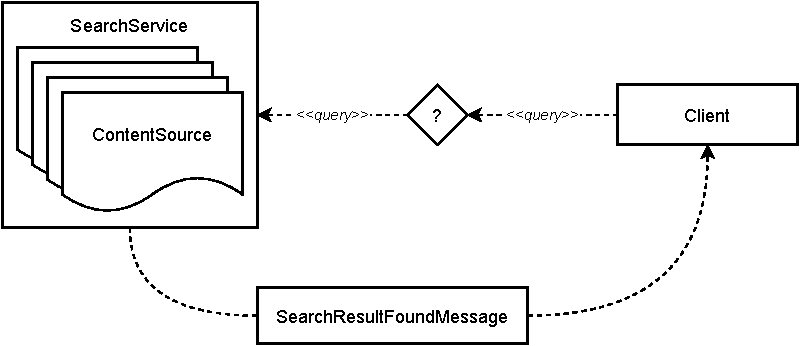
\includegraphics[scale=0.8]{figures/query_process.pdf}		
		\caption{Dinámica de las peticiones de búsqueda.}
	\end{figure}
	
	Sin embargo, como hemos mencionado anteriormente, \texttt{SearchService} solo provee un servicio de búsqueda, sin preocuparse de la concurrencia ni del encolado de las tareas. También vemos que esta solución nos limita a un único servicio de búsqueda, lo que impide que se atiendan a varios clientes de manera simultánea. Por este motivo, algún componente debe mediar entre el cliente y el servicio de búsqueda.
	
	\begin{figure}[h]
		\centering
		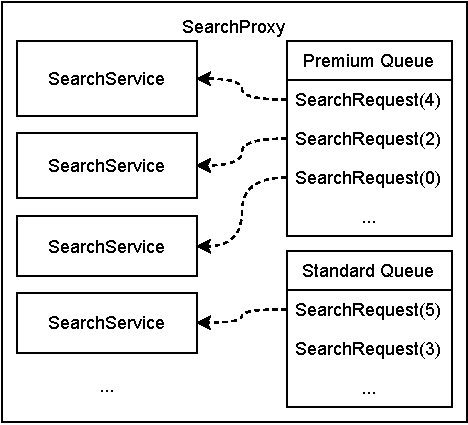
\includegraphics[scale=0.8]{figures/search_proxy.pdf}
		\caption{Clase \texttt{SearchProxy}.}
	\end{figure}
	
	La clase \texttt{SearchProxy} encapsula $N$ servicios de búsqueda (utilizando la función \texttt{std::thread::hardware\_concurrency()}, esto son tantos como núcleos lógicos tenga la plataforma) y dispone de dos colas de prioridad (que ordenan las peticiones de búsqueda de más antigua a más reciente según marca de tiempo de la petición): una para cada tipo de suscripción del cliente que realiza cada petición.
	
	De manera continua, el \textit{proxy} de búsqueda desencola peticiones de búsqueda y las asigna cada servicio de búsqueda disponible para que sean atendidas de manera paralela.
	
	\begin{quotation}
		\textbf{Política de desencolamiento.} Cada vez que se va a desencolar una petición, se sigue una función de distribución continua y uniforme para generar un número real arbitrario $p$ en el rango $[0, 1]$. Si $p\leq0.8$, se desencolará una petición de la cola \textit{premium}; de lo contrario, se desencolará de la cola estándar. Al ser una distribución uniforme, el 20\% de las veces se atendera a un cliente estándar y el 80\% restante a un cliente \textit{premium}. Es una solución \textit{na"if} a un problema de planificación que podría resolverse de manera más utilizando un algoritmo similar al de partición compartida (\textit{GPS} \cite{gps}) asignando un peso fijo a cada cola. Esto aseguraría que en todo momento se está atendiendo al 20\% de las peticiones estándar existentes y al 80\% de las peticiones \textit{premium} existentes. Por simplicidad, se ha implementado como se expone.
	\end{quotation}
	
	\subsection{Paso de Mensajes entre Componentes}
	Se pretende facilitar un mecanismo de comunicación simple a través del paso de mensajes que inician una operación atómica en el objeto que los recibe. Esto es útil para notificar a objetos de eventos a los que no se estaba esperando de forma activa (en contraste con otros que se explicarán más adelante) pero que deben incurrir en una acción inmediata.
	
	\begin{figure}[h]
		\centering
		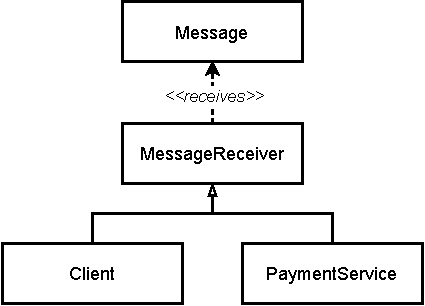
\includegraphics[scale=0.8]{figures/message_receivers.pdf}
		\caption{Clases \texttt{Client} y \texttt{PaymentService} derivadas de \texttt{MessageReceiver}.}
	\end{figure}
	
	Esta primitiva se utiliza principalmente para notificar a los clientes de la falta de saldo, la recarga de saldo, la ocurrencia de un resultado de búsqueda o la finalización de la búsqueda sin resultados. Varios objetos que implementen la interfaz \texttt{MessageReceiver} (\textit{receptores de mensajes}) pueden también enviarse mensajes entre sí\footnote{Eso sí, teniendo especial cuidado con la introducción de \textit{deadlocks} en la gestión de éstos.}, como es el caso de los clientes y el sistema de pago.
	
	Si bien cuando un cliente \textit{premium} agota todo su saldo disponible, es notificado mediante un mensaje \texttt{NotEnoughCreditMessage} por el servicio de búsqueda, el cliente responde notificando al servicio de pago a través de un mensaje de petición de recarga (\texttt{CreditRechargeRequestMessage}). El servicio de pago entonces remite una respuesta al cliente, tanto si se efectuó la recarga como si no, con la cantidad de créditos abonados (aunque hayan sido $0$).
	
	Las operaciones de gestión de mensajes son atómicas y deben ser breves. No deben ser abusadas para la implementación de esperas activas, como la que es necesaria para pausar y reanudar una búsqueda mientras el cliente recarga su saldo.
	
	\subsection{Espera Activa y Semáforos}
	Cuando un cliente agota todo su saldo, el servicio de búsqueda debe pausar la operación de búsqueda y esperar a que el saldo haya sido restaurado. Es tentador realizar una espera activa para solventar esto:
	
	\begin{verbatim}
		if (!client.has_credit() && client.is_premium())
		while (!client.has_credit);
	\end{verbatim}
	
	Sin embargo, hacerlo solo incurre un desaprovechamiento del tiempo de CPU asignado al hilo e introduce una fuga de recursos inaceptable. Necesitamos un mecanismo de señalización que nos permita esperar a que una condición se dé, como un \textit{semáforo}. La clase \texttt{Semaphore} implementa un semáforo binario utilizando la primitiva \texttt{std::condition\_variable} y nos ofrece una solución al problema de la pausa/reanudación de búsqueda.
	
	Cuando un cliente se queda sin saldo, se le envía el mensaje correspondiente para que solicite al servicio de pago una recarga. Un detalle importante de los mensajes es que pueden llevar \textit{estado}. Así, cuando se envía el mensaje, se envía con él una referencia al semáforo:
	
	\begin{verbatim}
		if (!client.has_credit() && client.is_premium()) {
		    Semaphore semaphore;
		    client.push_message(NotEnoughCreditMessage(semaphore));
		    semaphore.wait();
		}
	\end{verbatim}
	
	Cuando el cliente recibe el mensaje, envía al servicio de pago una solicitud de recarga a través de un mensaje con el mismo semáforo: 
	
	\begin{verbatim}
		void Client::push_message(NotEnoughCreditMessage &message)
		{
		    ps.push_message(CreditRechargeRequestMessage(*this, 15,
		    message.semaphore()));
		}
	\end{verbatim}
	
	Finalmente, el servicio de pago notifica la recarga a través de un mensaje y reanuda la búsqueda señalizando el semáforo (\texttt{semaphore.notify()}).
	
	\subsection{Algoritmo de Búsqueda y Paralelización}
	
	Cada vez que un servicio de búsqueda recibe una petición, $M$ hilos se encargan de ejecutar el algoritmo de búsqueda de manera concurrente sobre cada una de las fuentes de contenido registradas para la búsqueda (siendo $M$ el número de fuentes).
	
	\begin{quotation}
		\textbf{Observación.} Cada vez que un servicio de búsqueda va a atender una petición, crea hilos para cada fuente de contenido. Quizá sería más óptimo preasignar los hilos a cada fuente y notificar mediante un semáforo la entrada de una petición de búsqueda. Esperamos que no haya que implementar esto en una \textit{tercera} convocatoria.
	\end{quotation}
	
	El algoritmo de búsqueda itera sobre todas las líneas de texto de la fuente que se está procesando y realiza una transformación tanto en el término de búsqueda como en el texto para convertirlo a minúsculas y efectuar así una búsqueda insensible a mayúsculas (\textit{case-insensitive}).
	
	Por cada ocurrencia del término de búsqueda, se consume un crédito del cliente y se le notifica a través de un mensaje (\texttt{SearchResultFoundMessage}) con detalles sobre la línea, posiciones inicial y final, y las palabras que rodean al texto coincidente. Cuando un cliente estándar agota su saldo, no se realiza ninguna espera y el servicio de pago no realizará ninguna recarga efectiva (emitirá un mensaje de recarga con una cantidad de $0$ créditos).
	
	\begin{thebibliography}{9}
		\bibitem{arc}
		Automatic Reference Counting -- The Swift Programming Language Guide
		\\\textit{\hyperref{https://docs.swift.org/swift-book/LanguageGuide/AutomaticReferenceCounting.html}{}{}{https://docs.swift.org/swift-book/LanguageGuide/AutomaticReferenceCounting.html}}
		
		\bibitem{cppcon}
		CppCon 2017: Undefined Behaviour is awesome!--Piotr Padlewski
		\\\textit{\hyperref{https://isocpp.org/blog/2018/07/cppcon-2017-undefined-behaviour-is-awesome-piotr-padlewski}{}{}{https://isocpp.org/blog/2018/07/cppcon-2017-undefined-behaviour-is-awesome-piotr-padlewski}}
		
		\bibitem{gps}
		Generalized processor sharing -- Wikipedia
		\\\textit{\hyperref{https://en.wikipedia.org/wiki/Generalized\_processor\_sharing}{}{}{https://en.wikipedia.org/wiki/Generalized\_processor\_sharing}}
	\end{thebibliography}
\end{document}
